\documentclass[12pt]{beamer}
\usetheme{Boadilla}

\usepackage[utf8]{inputenc}
\usepackage{graphicx}
\usepackage{amsmath}
\usepackage{tikz}

\setbeamersize{text margin left=10mm,text margin right=10mm}

\title{Simulation Methods for Finance}
\subtitle{Barrier and Look-back Options}
\author{Espel, Kulak, Maclver, Qiu, Zhang}
\institute{Imperial College London}
\date{\today}

\begin{document}

\begin{frame}
    \titlepage
\end{frame}


\begin{frame}
\frametitle{Outline}
\tableofcontents
\end{frame}


\section{Random Variable Generation}

\begin{frame}
\frametitle{Random Variable Generation - Methods}
\begin{table}[]
\centering

\label{my-label}
\begin{tabular}{cc}
\textbf{Random}                              & \multicolumn{1}{l}{}      \\
\multicolumn{1}{l}{}                         & \multicolumn{1}{l}{}      \\
\textbf{Generate Uniform Distribution}       & \textbf{Convert U to SDN} \\
System built-in Rand & Central Limit Theory      \\
Linear Congruential Generator                & Box-Muller                \\
                                             & Marsagilia Polar
\end{tabular}
\end{table}

\end{frame}

\begin{frame}
\frametitle{Random Variable Generation - Analysis}
\begin{itemize}
\item Rand returns a random number in $(1, 2^{15}-1)$, may show correlation between numbers.\\
\item CLT requres a sufficient large number of uniform distributions, the computational time is long.\\
\item Box-Muller involves calculation of Sine Cosine and log. Computational time can be long.\\
\end{itemize}
\end{frame}


\begin{frame}
\frametitle{Random Variable Generation - Results}
Generating 100 million random numbers
\begin{center}
\begin{tabular}{| c| c| c| c| }
\hline
\textbf{ Method} &\textbf{ Mean} & \textbf{Variance}&\textbf{ Time} \\ \hline
\textbf{\textit{ rand}  + CLT} & 1.77 e-5 & 0.999909 & 90.34 \\  \hline
\textbf{\textit{ rand}  + Box-Muller} & -6.80 e-5 & 1.000703&8.64\\ \hline
\textbf{\textit{ rand}  + Marsagilia Polar} & 1.70 e-5& 1.000472& 6.40\\ \hline
\textbf{ LCG + CLT} & 1.52 e-5& 0.999973&236.3\\ \hline
\textbf{LCG + Box-Muller} & -1.27 e-4 & 0.999797&11.59\\ \hline
\textbf{ LCG + Marsagilia} & 7.36 e-5 & 0.999979&10.52\\ \hline
\textbf{\textit{Random} }& 3.58 e-4 & 1.000210&1.498\\ \hline

\end{tabular}
\end{center}

\end{frame}



\section{European Call Option}
\begin{frame}
\frametitle{European Call Option - Task}

With the usual conventions, recall our model.
$$dS_t=rS_tdt+\sigma S_tdW_t, \ 0\leq t \leq T$$
$$C_t = E[e^{-r(T-t)}(S_T-K)^+|\textit{F}_t]$$

\begin{itemize}
  \item Create a module to simulate the results for the European option.
  \item Compute the Greeks (delta, gamma, vega) using different methods.
  \item Analyse the error compared to the theoretical result.
\end{itemize}
\end{frame}

\begin{frame}
\frametitle{European Call Option - Analysis}
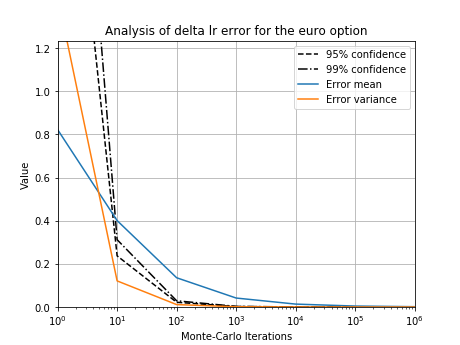
\includegraphics[width=.5\textwidth]{graphs/eurodeltalr.png}
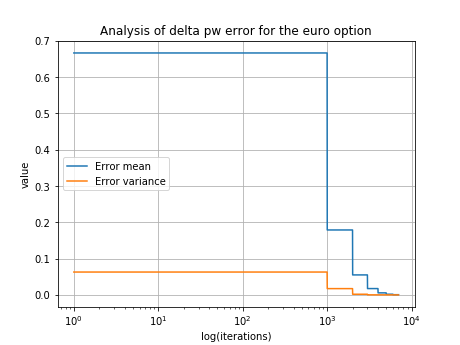
\includegraphics[width=.5\textwidth]{graphs/eurodeltapw.png}
\end{frame}

\begin{frame}
\frametitle{European Call Option - Analysis}
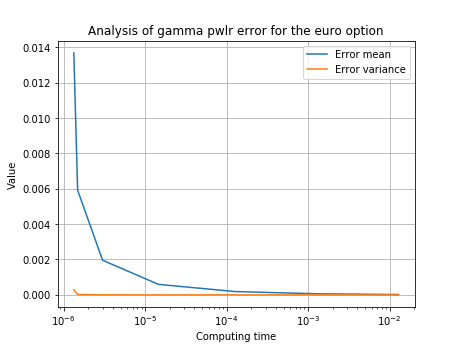
\includegraphics[width=.5\textwidth]{graphs/eurogammapwlrtime.png}
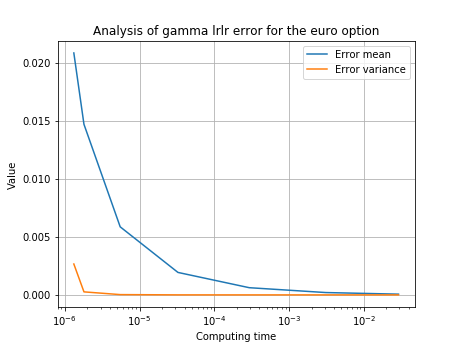
\includegraphics[width=.5\textwidth]{graphs/eurogammalrlrtime.png}
\end{frame}

\begin{frame}
\frametitle{European Call Option - Results}
\begin{itemize}
  \item There is a significant accuracy gap beyond 1,000 simulations.
  \item We based our conclusions on the industry standard: 100,000 simulations.
  \item There is a trade-off computation time/accuracy.
\end{itemize}



\begin{table}
  \centering
\begin{tabular}{|l|c|c|c|}
\hline
& \textbf{Error Mean} & \textbf{Error Variance} & \textbf{Time} \\ \hline
\textbf{Delta LR} & Worst & Worst & Best\\
\textbf{Delta PW} & Best & Best & Worst\\ \hline
\textbf{Gamma PWLR} & Worst & Best & Best\\
\textbf{Gamma LRPW} & - & Worst & Best\\
\textbf{Gamma LRLR} & - & - & Worst\\ \hline
\textbf{Vega LR} & Worst & - & Worst\\
\textbf{Vega PW} & Best & - & Best\\ \hline
\end{tabular}\\

\end{table}

\end{frame}




\section{Barrier Option}
\begin{frame}
\frametitle{Barrier Option - Task}
$$m^T_{0} =\underset{0 \leq t \leq T}{min}  S_t, \ \   M^T_{0} = \underset{0 \leq t \leq T}{max} S_t$$\\

For an up-and-out barrier call option, $B > S_0$ $A_T=(S_T-K)^+1_{M^T_0 < B}$, where $B$ is a barrier level and $1_S$ is an indicator function.

\end{frame}

\section{Barrier Option}
\begin{frame}
\frametitle{Barrier Option - Two Methods}

1. Generate whole paths of $S_t$ with 1,000 stops each path.\\

Time used for ***simulation : ***seconds/minutes/hours

\end{frame}

\begin{frame}
\frametitle{Barrier Option - Two Methods}

2. Use Rayleigh distribution generate the $M_T$ directly. \\
The maximum of a standard Brownian motion starting at the origin to be at b at time 1 over period [0, T] has the Rayleigh distribtuion

$$F(x) = 1 - e^{-2x(x-b)}, \ x \geq b.$$
Hense, at time T with $S_T$,
$$M^T={S_T+\sqrt{S_T^2-2TlogU}\over 2}$$

Method 2 is 500 times faster!

\end{frame}

\begin{frame}
\frametitle{Barrier Option - Analysis}
%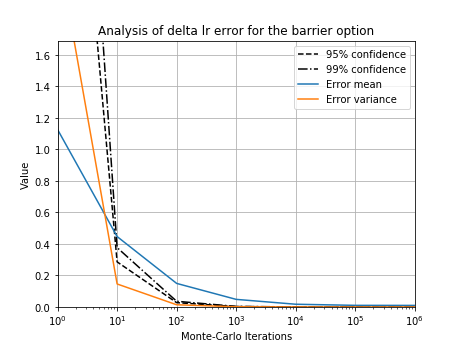
\includegraphics[width=.5\textwidth]{graphs/barrierdeltalr.png}
%\includegraphics[width=.5\textwidth]{graphs/barriergammalr.png}
Simulate Greeks using Likelihood ratio method as Pathwise method is not feasible for barrier option.


\end{frame}

\begin{frame}
\frametitle{Barrier Option - Analysis with a New Method}
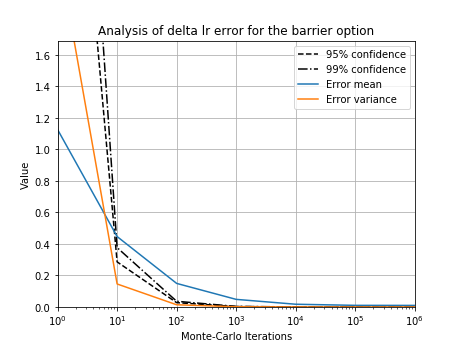
\includegraphics[width=.5\textwidth]{graphs/barrierdeltalr.png}
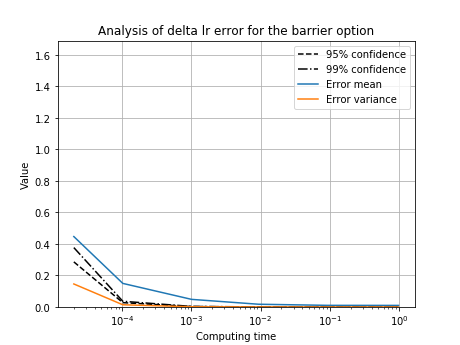
\includegraphics[width=.5\textwidth]{graphs/barrierdeltalrtime.png}
\end{frame}

\begin{frame}
\frametitle{Barrier Option - Analysis with a New Method}
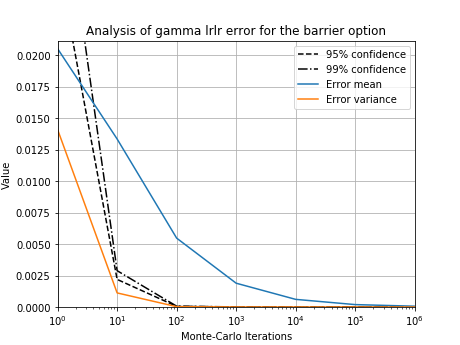
\includegraphics[width=.5\textwidth]{graphs/barriergammalrlr.png}
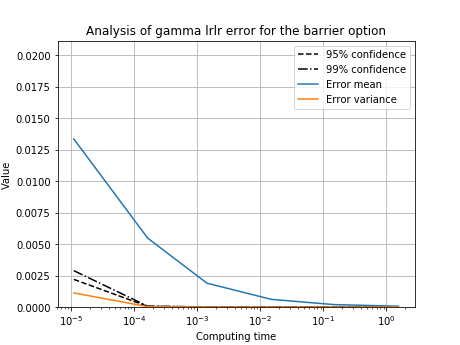
\includegraphics[width=.5\textwidth]{graphs/barriergammalrlrtime.png}
\end{frame}

\begin{frame}
\frametitle{Barrier Option - Results}
\begin{table}
\centering
\begin{tabular}{|l|c|c|c|}
\hline
    & \textbf{Error Mean} & \textbf{Error Variance} & \textbf{Time (s)} \\ \hline
\textbf{Price} & na &          na         & .. \\ \hline
\textbf{Delta LR} & 1.04 e-2 & 3.03 e-5 & 9.28 e-2\\ \hline
\textbf{Gamma LRLR} & 1.89 e-4 & 1.89 e-8& 1.48 e-1\\ \hline
\textbf{Vega LR} & 7.51 e-1 & 3.22 e-1 & 1.09 e-1\\ \hline
\end{tabular}
\caption{Sample from our simulation dataset with the new fast method for barrier option simulation. It is clear that the results have significantly improved compared with the previous method. note that the run time depends on the computer used (here a 3.4 GHz Intel Core i7).}
\end{table}

\end{frame}


\section{Look-back Option}
\begin{frame}
\frametitle{Look-back Option - Task}
Lookback call option with fixed strik price $K$ has payoff $(M^T_{0}-K)^+$. The call option price at time $t$ is

$$c(S_0,K,t) = e^{-r(T-t)}E[(max(M^t_0,M^T_t)-K)^+|\mathcal{F}_t] $$


\end{frame}

\begin{frame}
\frametitle{Look-back Option - Method}
The cdf of the distribution of Maximum $S_t$ for standard Brownian motion for the period of (0, T) is

$$F = \Phi(\frac{m-aT}{\sqrt{T}})-e^{2am}\Phi(\frac{-m-aT}{\sqrt{T}})$$

We used Newton-Raphson method to solve for the above cdf F = U. Hense, for each random number we generate from [0,1], we receive one m in by solving for F. And to get $M^T$ of stock price follows geometric Browninan motion with starting price $S_0$, we let $M^T=S_0e^{\sigma m }$.\\


\end{frame}

\begin{frame}
\frametitle{Look-back Option - Analysis}
%\includegraphics[width=.5\textwidth]{graphs/lookbdeltalr.png}
%\includegraphics[width=.5\textwidth]{graphs/lookbgammalr.png}
\end{frame}

\begin{frame}
\frametitle{Look-back Option - Results}

\end{frame}


\section{Using our Code}
\begin{frame}
\frametitle{Using our Code - C++ Package}
\begin{itemize}
  \item We have created a package for C++ users.
  \item Uses industry standards with dynamic library files.
  \item Package is very intuitive.
\end{itemize}

\begin{figure}[h!]
  \centering
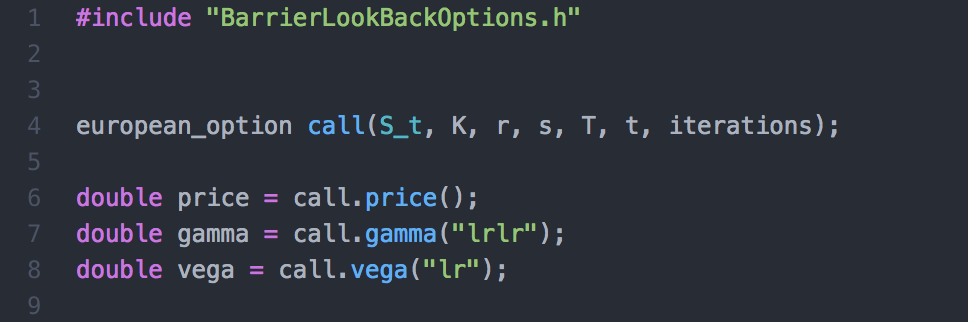
\includegraphics[width=\textwidth]{graphs/code_easy_demo.png}
\end{figure}
\end{frame}


\begin{frame}
\frametitle{Using our Code - "Code Free" terminal}
\begin{itemize}
  \item We have created an intuitive interface.
  \item This is suitable for users who do not code: you just have to type the command and there is a help mode.
  \item It supports european call option, barrier out call option and the look-back call option price and greeks.
\end{itemize}
\begin{figure}[h!]
  \centering
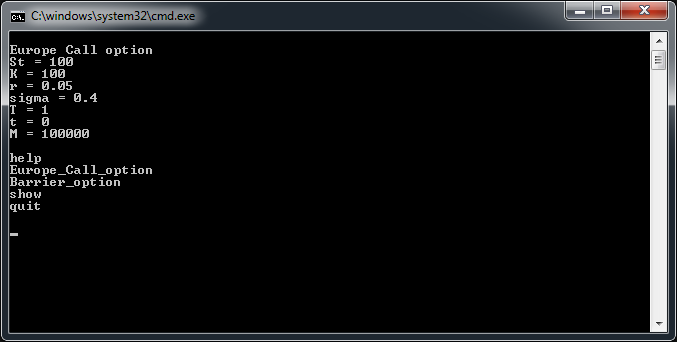
\includegraphics[width=.8\textwidth]{graphs/interface_demo.png}
\end{figure}
\end{frame}



\begin{frame}
\frametitle{Conclusion}
\begin{itemize}
  \item We have created a module with the core task.
  \item The module also can also compute elements related to the barrier option and the look-back option.
  \item Our package is user-friendly and has a "code-free" interface.
\end{itemize}
\end{frame}



\begin{frame}

\centering
{\Large Thank you!}
\\[1cm]
{\small\url{github.com/tjespel/barrier-and-look-back-options}}
\end{frame}

\end{document}
